\documentclass[11pt]{article}
\usepackage[margin=1in]{geometry}
\usepackage{amsmath,amssymb,booktabs,graphicx}

\title{\textbf{MECH559: Assignment 1} \\ Quadrotor Optimization}
\author{Lucas Bessai, 261050265 \\ \small{Department of Mechanical Engineering, McGill University} \\ \small{817 Sherbrooke Street West, Montreal, QC, H3A 0C3}}
\date{\today}

\begin{document}

\maketitle

\tableofcontents

\section{Homework 1: Simple Drone Design Optimization}
The design variables are the rotor radius and arm length,
\begin{equation}
 \mathbf{x}=\begin{bmatrix}R & L\end{bmatrix}^{T}.
\end{equation}
All other quantities are treated as fixed parameters.

\section{Part (a): Formulation in negative-null form}

\subsection{Selected parameters}
The arms are modeled as solid circular aluminum bars. Table~\ref{tab:parameters} gives the parameter set used by the Python implementation. The stress limit is treated as an allowable stress for this assignment.

\begin{table}[h]
\centering
\caption{Fixed parameters used in the formulation.}
\label{tab:parameters}
\begin{tabular}{lll}
\toprule
Parameter & Value & Description \\
\midrule
$r$ & $5~\mathrm{mm}$ & Arm radius \\
$\phi$ & $90^\circ$ & Inter-arm angle \\
$m_0$ & $1.0~\mathrm{kg}$ & Fixed drone mass, excluding arms \\
$\rho$ & $1.225~\mathrm{kg/m^3}$ & Air density \\
$\rho_{\mathrm{mat}}$ & $1600~\mathrm{kg/m^3}$ & Arm density \\
$E$ & $70~\mathrm{GPa}$ & Young's modulus \\
$P_0$ & $1000~\mathrm{W}$ & Rated electrical power per motor \\
$\eta$ & $0.80$ & Electrical-to-aerodynamic power efficiency \\
$\sigma_y$ & $250~\mathrm{MPa}$ & Maximum allowable stress \\
$\delta_{\max}$ & $5~\mathrm{mm}$ & Maximum allowable tip deflection \\
$k$ & $1.5$ & Required thrust-margin factor \\
$g$ & $9.81~\mathrm{m/s^2}$ & Gravitational acceleration \\
\bottomrule
\end{tabular}
\end{table}

For convenience, define the positive constant
\begin{equation}
 C_T=\left(\eta P_0\sqrt{2\rho\pi}\right)^{2/3}>0.
\end{equation}
The thrust of each rotor is then
\begin{equation}
 T(R)=C_T R^{2/3}.
\end{equation}
The arm mass, total mass, maximum bending stress, and tip deflection are
\begin{align}
 W(L) &=4\rho_{\mathrm{mat}}\pi r^2L, \\
 m(L) &=m_0+W(L), \\
 \sigma_{\max}(R,L)&=\frac{4C_TR^{2/3}L}{\pi r^3}, \\
 \delta(R,L)&=\frac{4C_TR^{2/3}L^3}{3\pi Er^4}.
\end{align}

The optimization problem is therefore
\begin{align}
 \underset{R,L}{\operatorname{minimize}}\quad & W(R,L)=4\rho_{\mathrm{mat}}\pi r^2L \\
 \text{subject to}\quad
 g_1(R,L)&=R-\frac{L}{\sqrt{2}}\leq0 && \text{(rotor clearance)},\\
 g_2(R,L)&=\frac{4C_TR^{2/3}L}{\pi r^3}-\sigma_y\leq0 && \text{(bending stress)},\\
 g_3(R,L)&=\frac{4C_TR^{2/3}L^3}{3\pi Er^4}-\delta_{\max}\leq0 && \text{(tip deflection)},\\
 g_4(R,L)&=k\left(m_0+4\rho_{\mathrm{mat}}\pi r^2L\right)g-4C_TR^{2/3}\leq0 && \text{(thrust margin)},\\
 &R\geq0,\quad L\geq0. && \text{(physical variable bounds)}
\end{align}
The last constraint is equivalent to $4T(R)\geq k m(L)g$ and correctly uses the thrust from all four rotors.

\section{Part (b): Monotonicity and well-posedness}

\subsection{Monotonicity table}
For the physically relevant interior domain $R>0$ and $L>0$, monotonicity follows from the signs of the partial derivatives. For example,
\begin{align}
 \frac{\partial g_2}{\partial R}
 &=\frac{8C_TL}{3\pi r^3}R^{-1/3}>0, &
 \frac{\partial g_2}{\partial L}
 &=\frac{4C_TR^{2/3}}{\pi r^3}>0,\\
 \frac{\partial g_4}{\partial R}
 &=-\frac{8C_T}{3}R^{-1/3}<0, &
 \frac{\partial g_4}{\partial L}
 &=4k\rho_{\mathrm{mat}}\pi r^2g>0.
\end{align}
The corresponding table is shown in Table~\ref{tab:monotonicity}. A plus sign means that increasing the variable increases the function and hence moves a negative-null constraint closer to violation. A minus sign has the opposite effect.

\begin{table}[h]
\centering
\caption{Monotonicity of the objective and constraints for $R,L>0$.}
\label{tab:monotonicity}
\begin{tabular}{lcc}
\toprule
Function & $R$ & $L$ \\
\midrule
$W$ (arm mass) & & $+$ \\
$g_1$ (clearance) & $+$ & $-$ \\
$g_2$ (stress) & $+$ & $+$ \\
$g_3$ (deflection) & $+$ & $+$ \\
$g_4$ (thrust margin) & $-$ & $+$ \\
\bottomrule
\end{tabular}
\end{table}

\subsection{Interpretation}
The objective is independent of $R$ and strictly increasing in $L$; consequently, a mass-minimizing optimizer always attempts to reduce $L$. The physics prevents the apparently problematic limit $L\to0$:
\begin{enumerate}
 \item The clearance constraint requires $L\geq\sqrt{2}R$.
 \item If $R\to0$, then $T(R)\to0$, whereas $k m(L)g>0$ because $m_0>0$. Thus $g_4>0$, which violates the thrust-margin constraint.
 \item Hence thrust imposes a positive lower limit on $R$, and clearance transfers that lower limit to $L$. In particular, the thrust constraint can be rearranged as
 \begin{equation}
 R\geq\left[\frac{kg\left(m_0+4\rho_{\mathrm{mat}}\pi r^2L\right)}{4C_T}\right]^{3/2}.
 \end{equation}
\end{enumerate}
Therefore $W$ cannot be driven to zero while maintaining feasibility in the physical first quadrant. The likely optimum lies on the lower feasible boundary, commonly where the clearance and thrust-margin constraints are both active. Stress and deflection need not be active at the optimum for the selected parameters, but they restrict overly large designs.

The feasible region is also bounded above once the physical bounds are imposed. Clearance gives $L\geq\sqrt{2}R$, so along any sequence with $R\to\infty$, the stress term behaves at least as $R^{2/3}(\sqrt{2}R)=\mathcal{O}(R^{5/3})$ and eventually violates $g_2\leq0$. A sequence with $L\to\infty$ violates $g_2$, $g_3$, and also makes $g_4$ increase through arm mass. Thus, if the selected numerical parameters admit a solution, the feasible set is contained within finite positive ranges of $R$ and $L$.

The explicit bounds $R\geq0$ and $L\geq0$ are nevertheless essential. Without them, negative lengths are permitted algebraically even though they are physically meaningless. Taking both $R$ and $L$ to large negative values can satisfy the written inequality forms while making $W\propto L$ arbitrarily negative. The physics-derived inequalities alone would then not make the optimization problem well-posed. With the nonnegative physical bounds, the thrust and clearance constraints automatically exclude the zero-size design, and the problem has a finite lower objective bound.

\section{Part (c): Numerical solution}

The problem was solved with the SLSQP constrained optimizer from
\texttt{scipy.optimize}. The initial point was $(R,L)=(0.05,0.10)$ m. The
optimizer returned a successful solution after 10 iterations.

\begin{table}[h]
\centering
\caption{Numerical optimum for the nominal parameter set.}
\label{tab:nominal-result}
\begin{tabular}{lll}
\toprule
Quantity & Value & Units \\
\midrule
$R^*$ & $0.003190$ & m \\
$L^*$ & $0.004511$ & m \\
$W(L^*)$ & $0.002268$ & kg \\
$m(L^*)$ & $1.002268$ & kg \\
$T(R^*)$ & $3.687$ & N per rotor \\
\bottomrule
\end{tabular}
\end{table}

The optimum is controlled by the thrust-margin and clearance constraints. Their
normalized values are approximately zero:
\begin{equation}
 g_4=5.3\times10^{-15}, \qquad g_1=-1.7\times10^{-12}.
\end{equation}
The small numerical differences from zero are solver tolerances. The stress and
deflection constraints are safely inactive. The maximum stress is
$169{,}425$ Pa, compared with the $250$ MPa limit, and the tip deflection is
$3.28\times10^{-9}$ m, compared with the $5$ mm limit.

Figure~\ref{fig:objective} shows the objective over the design space. Figure~\ref{fig:design-space}
shows the feasible region and all constraint boundaries. The optimum occurs at
the intersection of the clearance and thrust-margin boundaries. Since arm mass
increases with $L$, the optimizer selects the smallest arm length that can still
provide the required thrust.

\begin{figure}[h!]
\centering
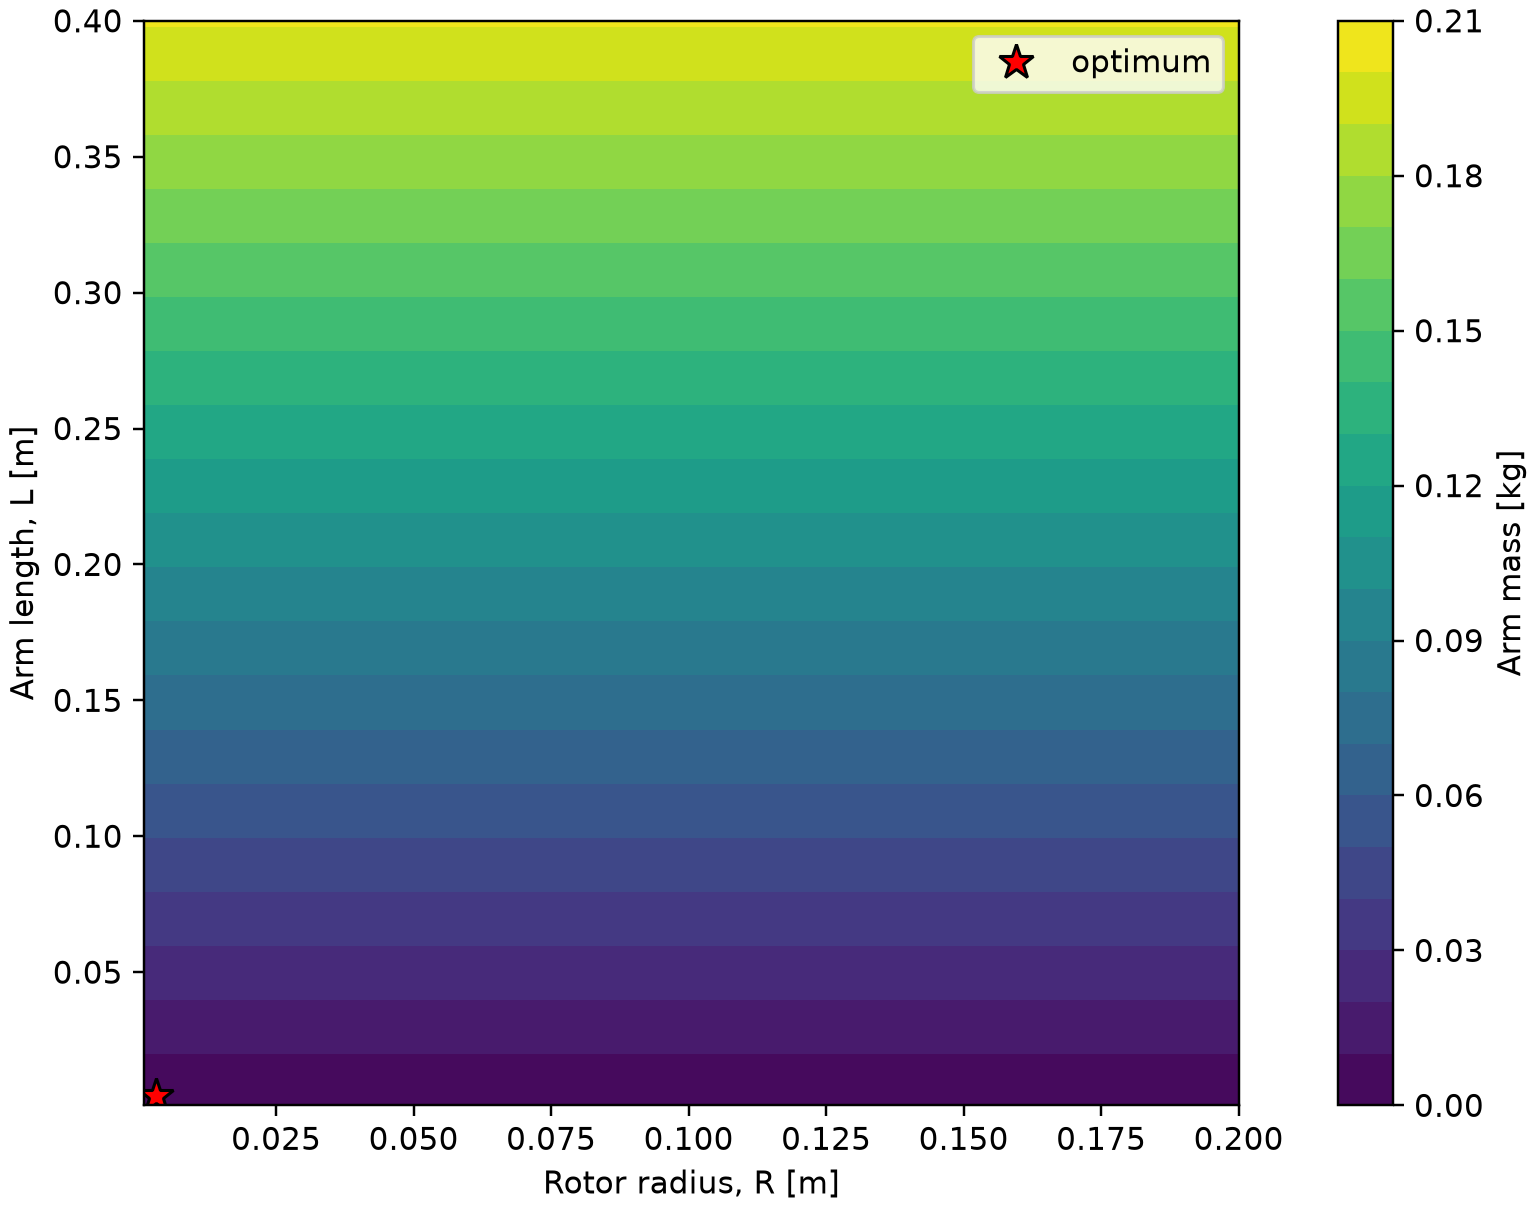
\includegraphics[width=0.78\textwidth]{figures/objective_contour.png}
\caption{Arm-mass objective over the design space.}
\label{fig:objective}
\end{figure}

\begin{figure}[h!]
\centering
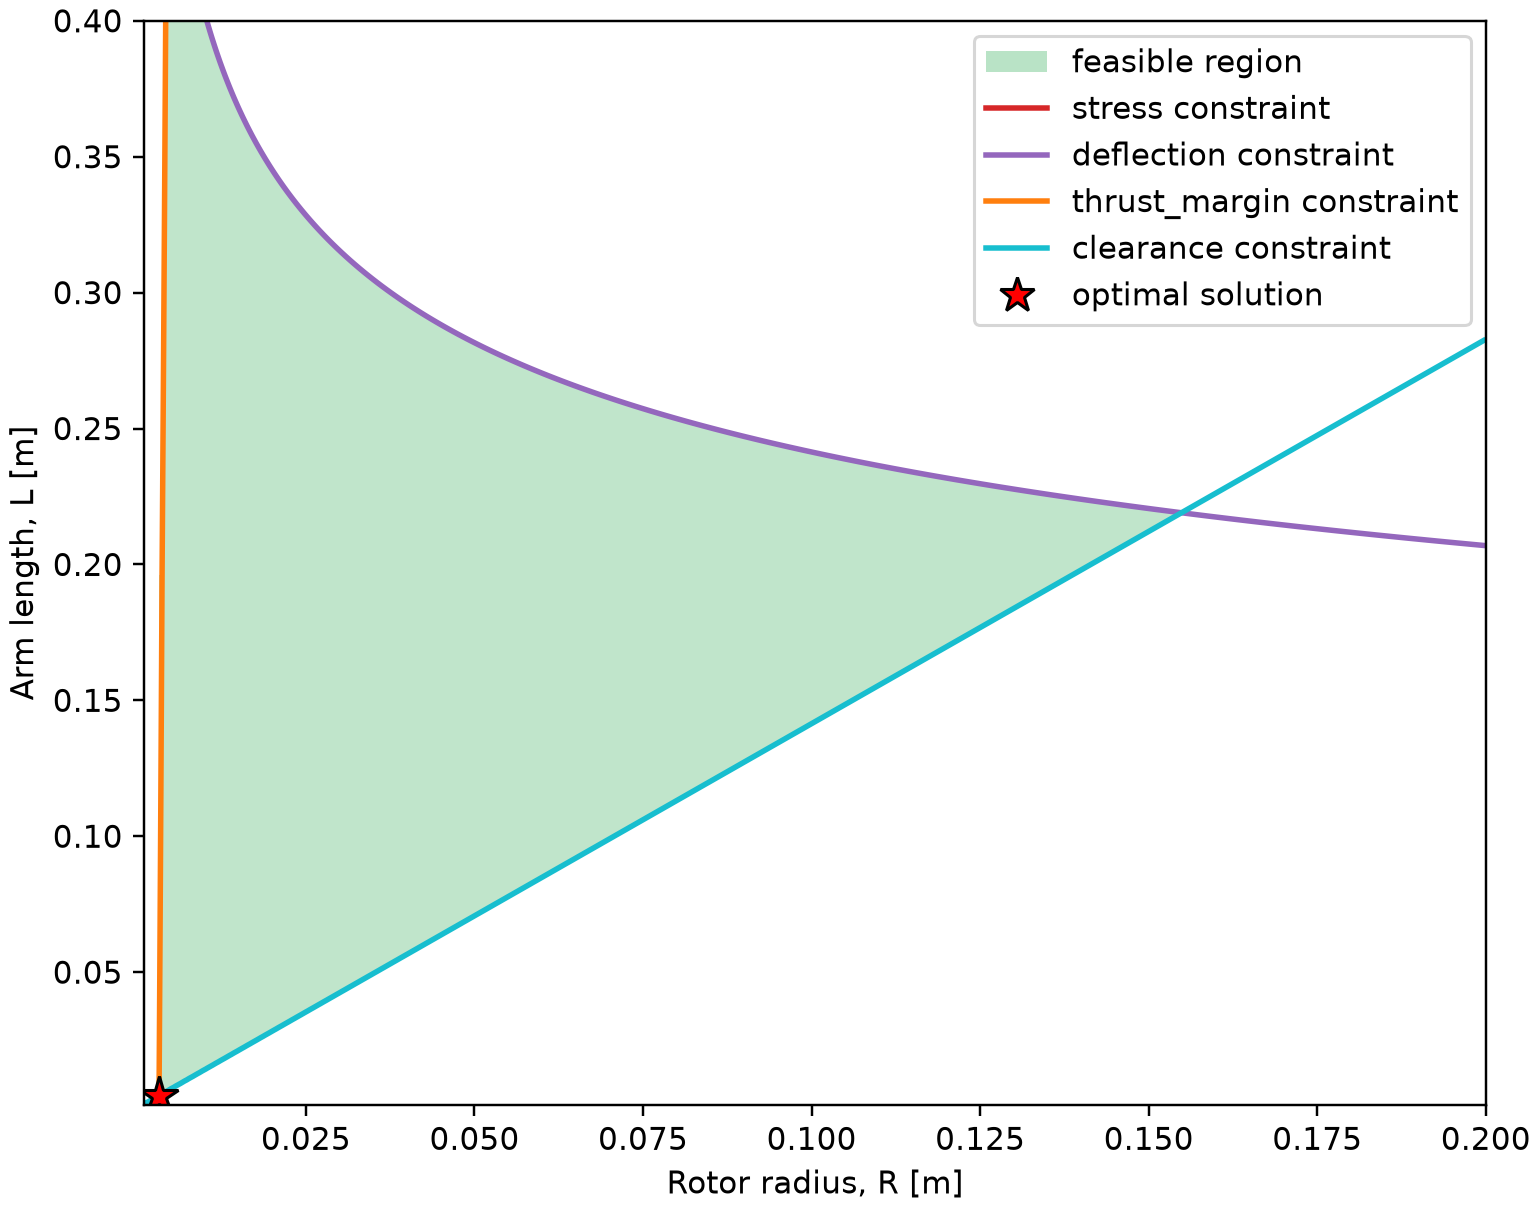
\includegraphics[width=0.78\textwidth]{figures/constrained_design_space.png}
\caption{Constrained design space. The green region is feasible.}
\label{fig:design-space}
\end{figure}

\section{Part (d): Parameter studies}

Two parameter studies were performed. First, the rated motor power was changed
to 700, 1000, and 1300 W. Second, the required thrust-margin factor was changed
from $k=1$ to $k=10$. For each case, the optimization was solved again from the
same initial point.

Increasing motor power reduces the required rotor radius and arm length. The
arm mass decreases from $3.24$ g at 700 W to $1.74$ g at 1300 W. More motor
power allows the required thrust to be produced with a smaller rotor.

Increasing $k$ has the opposite effect. The optimal arm mass increases from
$1.23$ g at $k=1$ to $41.34$ g at $k=10$. In every case, the thrust-margin and
clearance constraints are active, while stress and deflection remain inactive.

\begin{figure}[h!]
\centering
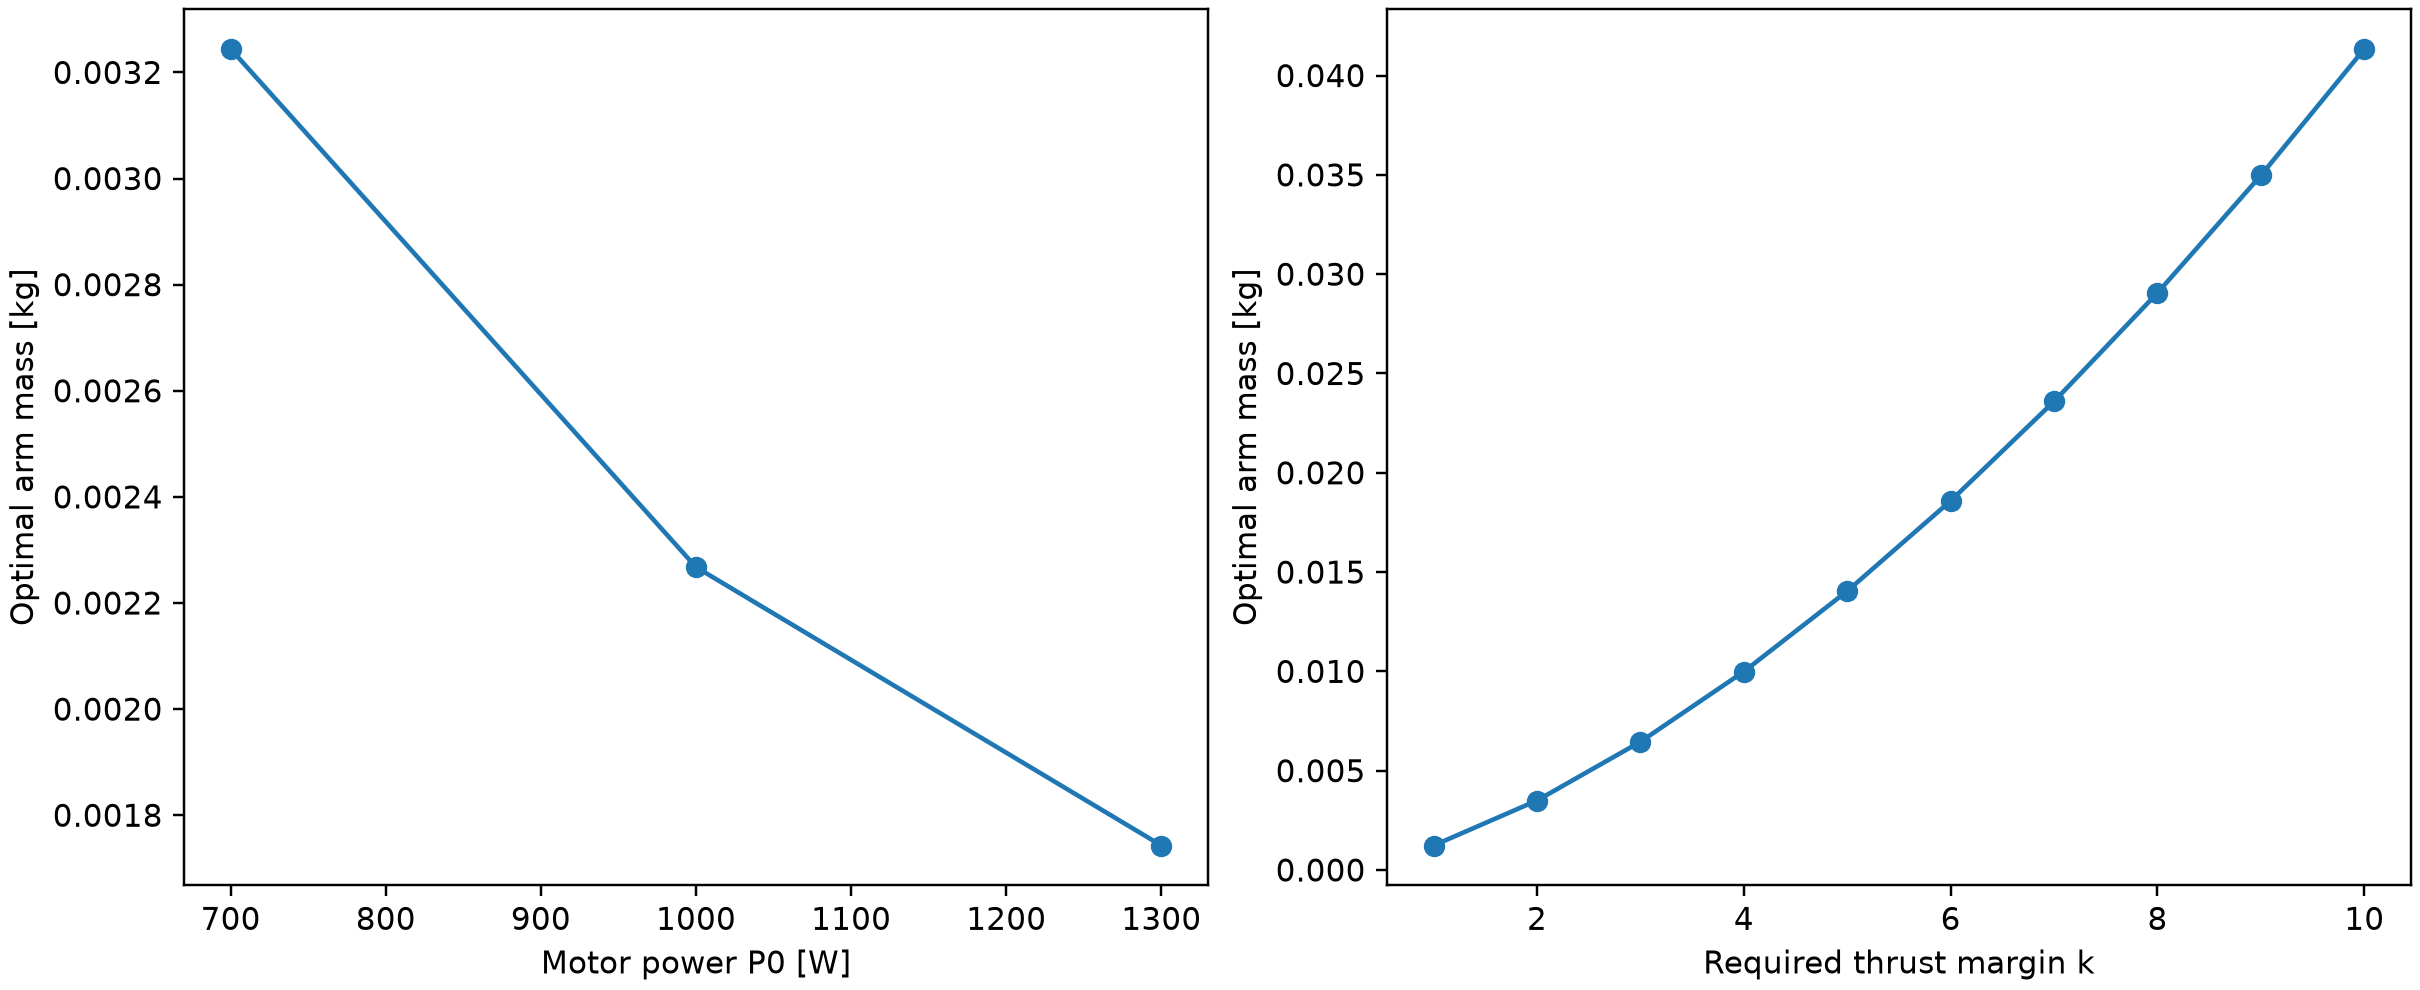
\includegraphics[width=0.82\textwidth]{figures/parameter_sweeps.png}
\caption{Effect of motor power and thrust-margin factor on optimal arm mass.}
\label{fig:sweeps}
\end{figure}

Figure~\ref{fig:k-sweep} plots the optimal $(R,L)$ pair for every value of $k$.
The points move along the clearance boundary as the required thrust margin
increases. The faint lines show the constraint boundaries for each value of
$k$. Figure~\ref{fig:k-sweep-all} also shows the inactive stress and deflection
boundaries. These boundaries are far from the optimum over the selected range.

\begin{figure}[h!]
\centering
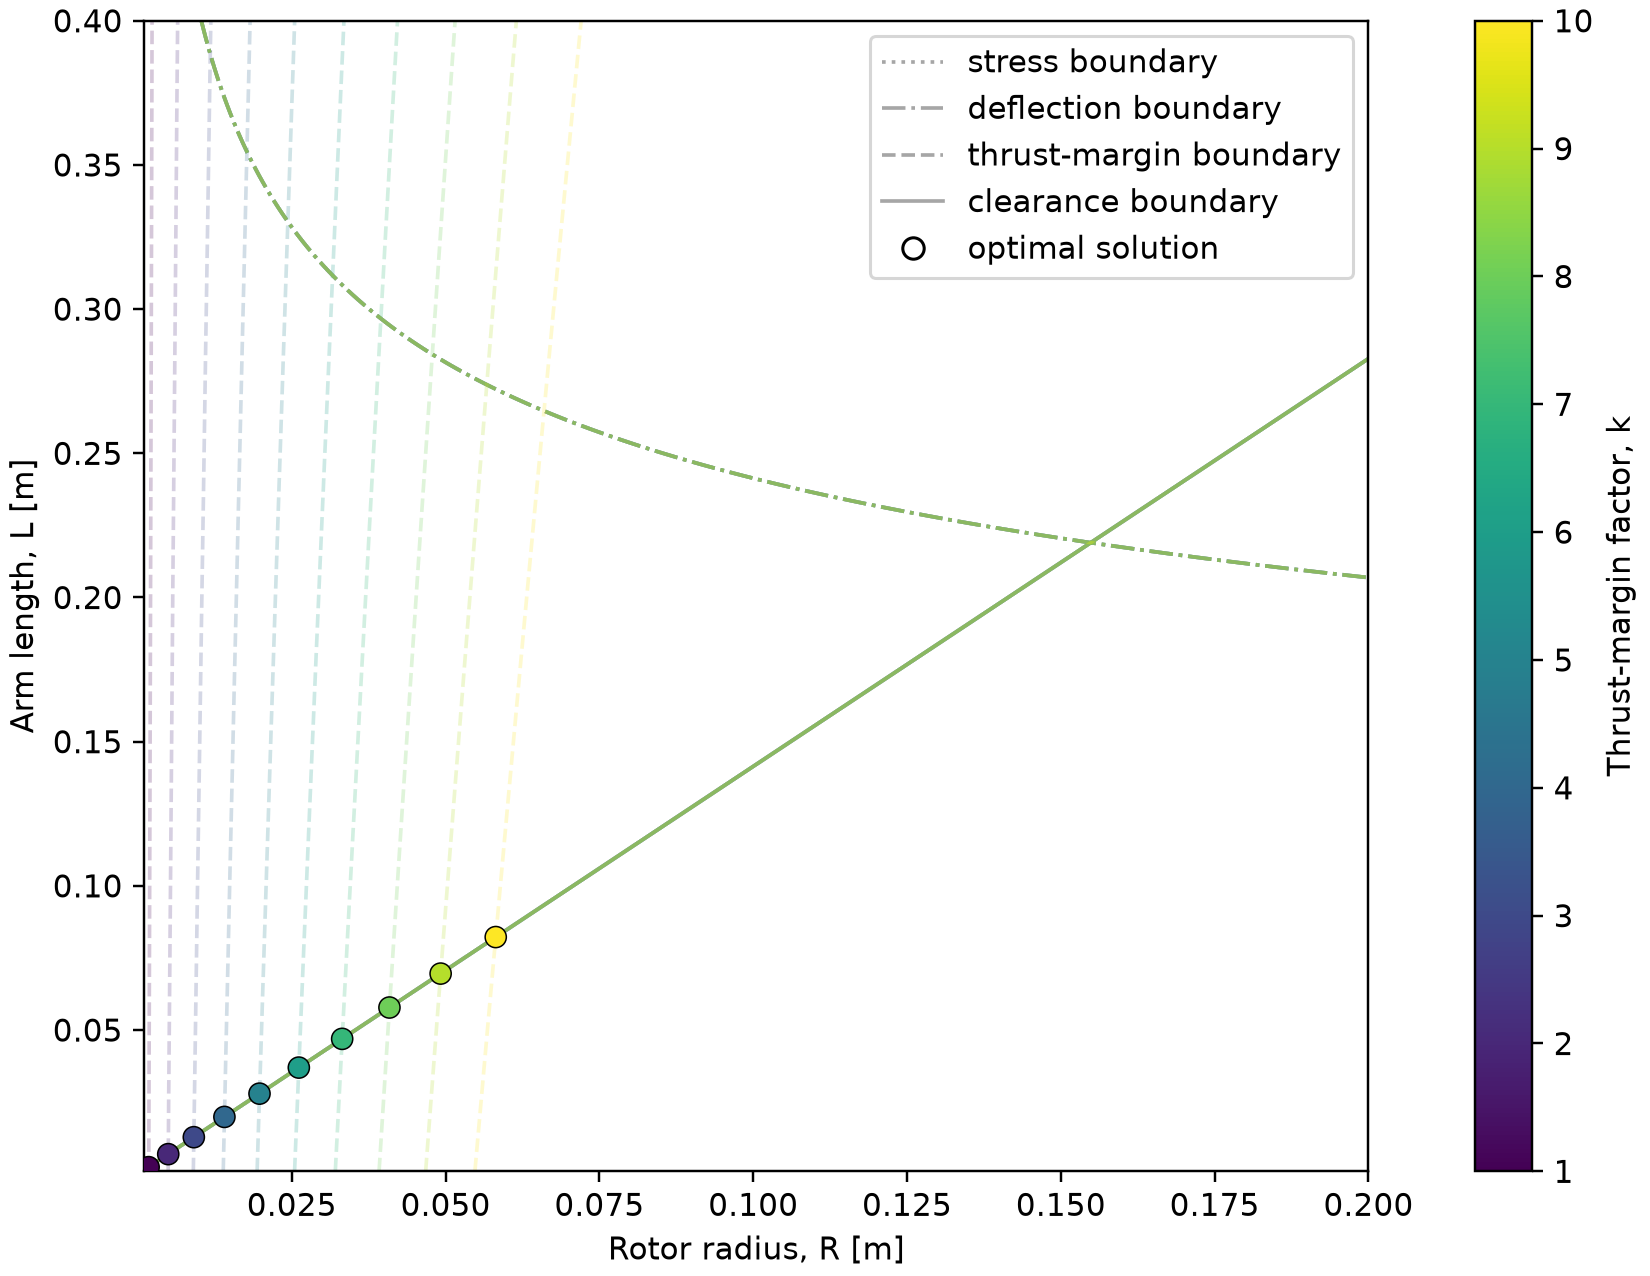
\includegraphics[width=0.82\textwidth]{figures/k_sweep_design_space_all_constraints.png}
\caption{Optimal designs and all constraint boundaries for $k=1$ to $10$.}
\label{fig:k-sweep-all}
\end{figure}

\section{Bonus: Which constraints govern the design?}

The numerical results show that the thrust-margin and clearance constraints
govern the optimum. This follows directly from the structure of the problem:
the objective increases with arm length, so the optimizer tries to reduce $L$.
The clearance constraint then limits how small $L$ can be for a given rotor
radius, while the thrust-margin constraint sets the minimum rotor radius needed
to support the drone.

The stress constraint leaves substantial additional design capacity. At the
largest investigated value, $k=10$, the optimized stress is only about $8.6\%$
of the allowable stress. Along the clearance boundary, the stress limit would
be reached at approximately
\begin{equation}
 R\approx0.385~\mathrm{m}, \qquad L\approx0.272~\mathrm{m},
\end{equation}
for the selected fixed parameters. This corresponds to a supported thrust
margin of approximately $k=32.3$, well beyond the plotted range.

Thus, the current design is not strength-limited. It is primarily a thrust and
geometric-clearance design. The deflection constraint is even less restrictive
than the stress constraint for the selected arm radius and material.

The main modeling conclusion is that changing the structural limits would have
almost no effect on the reported optimum unless they were made much tighter.
Changing motor power or the required thrust margin has a direct and visible
effect because those parameters determine the minimum rotor size.

\end{document}
